%%%%%%%%%%%%%%%%%%%%%%%%%%%%%%%%%%%%%%%%%%%%%%%%%%%%%%%%%%%%%%%%%%%%%%%%
% MMSAR Conference Paper (ICSPIS 2026)
% IEEE Conference Template (Two-Column, Strictly <= 6 Pages)
%%%%%%%%%%%%%%%%%%%%%%%%%%%%%%%%%%%%%%%%%%%%%%%%%%%%%%%%%%%%%%%%%%%%%%%%
\documentclass[conference]{IEEEtran}
\IEEEoverridecommandlockouts

\usepackage{cite}
\usepackage{amsmath,amssymb,amsfonts}
\usepackage{algorithm}
\usepackage{algorithmic}
\usepackage{graphicx}
\usepackage{textcomp}
\usepackage{xcolor}
\usepackage{booktabs}
\usepackage{url}
\usepackage{balance}
\usepackage{placeins}
\usepackage{tikz}
\usepackage{pgfplots}

\pgfplotsset{compat=1.18}
\usetikzlibrary{arrows.meta,positioning,shapes.geometric,calc,fit,backgrounds,decorations.pathreplacing,plotmarks}

% Declare custom pentagon* plotmark used in figure_performance_tradeoff.tex
\pgfdeclareplotmark{pentagon*}{%
  \pgfpathmoveto{\pgfpointpolar{90}{\pgfplotmarksize}}%
  \pgfpathlineto{\pgfpointpolar{162}{\pgfplotmarksize}}%
  \pgfpathlineto{\pgfpointpolar{234}{\pgfplotmarksize}}%
  \pgfpathlineto{\pgfpointpolar{306}{\pgfplotmarksize}}%
  \pgfpathlineto{\pgfpointpolar{18}{\pgfplotmarksize}}%
  \pgfpathclose
  \pgfusepathqfillstroke
}

\setlength{\textfloatsep}{5pt plus 1pt minus 1pt}
\setlength{\floatsep}{4pt plus 1pt minus 1pt}
\setlength{\intextsep}{4pt plus 1pt minus 1pt}
\setlength{\abovecaptionskip}{2pt plus 1pt minus 1pt}
\setlength{\belowcaptionskip}{1pt plus 1pt minus 1pt}

\begin{document}

\title{Causal Temporal Filtering for Reliable Alerts in Multimodal UAV Search and Rescue Detection}
\author{\IEEEauthorblockN{1\textsuperscript{st} Oumar Mamoun Ibrahim}
\IEEEauthorblockA{\textit{Department of Computer Engineering} \\
\textit{University of Sharjah}\\
Sharjah, UAE \\
U22200741@sharjah.ac.ae}
\and
\IEEEauthorblockN{2\textsuperscript{nd} Mohamad Khairi bin Ishak}
\IEEEauthorblockA{\textit{Department of Computer Engineering} \\
\textit{University of Sharjah}\\
Sharjah, UAE \\
mishak@sharjah.ac.ae} 
}

\maketitle

\begingroup
\renewcommand\thefootnote{}
\footnotetext{No human subjects were involved; all imagery is synthetically generated.}
\endgroup

\begin{abstract}
Autonomous unmanned aerial vehicles (UAVs) in wilderness search and rescue (SAR) require reliable person alerts under strict Size, Weight, Power, and Cost (SWaP-C) limits, where per-frame detector fluctuations can trigger costly loiter maneuvers. We investigate whether learned temporal sequence models are necessary to convert noisy multimodal detections into reliable alerts, or whether simple causal filters suffice. On a controlled benchmark spanning arid desert, temperate forest, and snow alpine biomes with synchronized visible RGB and pseudo-TIR streams, fixed Ultralytics YOLO11n detectors feed a late-fusion max gate and a five-frame causal decision window (208~ms span at 24~Hz). We compare raw thresholding, moving average, median filtering, history consensus, a Mamba selective state-space model (SSSM), and a gated recurrent unit (GRU). A five-frame moving average reduces false alerts by 77\% (9.0 to 2.1 per minute) at 84.6\% recall, while a five-frame median filter preserves baseline recall (92.3\%, 12/13 tiles) at 291.7~ms latency with 3.6 false alerts per minute. Small Mamba-SSSM and GRU models trained on this scalar stream yield no statistically significant alert-reliability gain despite $73\times$--$500\times$ higher computational cost. Lightweight causal filtering therefore provides a practical, training-free baseline for edge SAR avionics.
\end{abstract}

\begin{IEEEkeywords}
object detection, edge computing, search and rescue, unmanned aerial vehicles, temporal filtering.
\end{IEEEkeywords}

\begin{figure*}[!t]
\centering
\resizebox{1.0\textwidth}{!}{\begin{tikzpicture}[
>=Stealth,
font=\sffamily\small,
box/.style={draw=black!70, rounded corners=3pt, thick, fill=white, align=center},
iconbox/.style={draw=none, fill=none, align=center, inner sep=1pt},
videobox/.style={draw=blue!60!black, rounded corners=3pt, thick, fill=black!2, align=center, inner sep=2.5pt},
framebox/.style={draw=teal!60!black, rounded corners=3pt, thick, fill=white, align=center, inner sep=2.5pt},
stepbox/.style={box, fill=green!12, draw=green!60!black, thick, font=\sffamily\scriptsize, align=center},
detector/.style={box, fill=cyan!10, draw=cyan!70, font=\sffamily\footnotesize, text width=2.6cm, minimum height=1.15cm},
fusion/.style={box, fill=purple!10, draw=purple!70, thick, font=\sffamily\footnotesize, text width=2.5cm, minimum height=1.1cm},
method/.style={box, fill=orange!10, draw=orange!75, thick, font=\sffamily\scriptsize, text width=3.7cm, inner ysep=5pt, inner xsep=7pt},
decision/.style={box, fill=teal!12, draw=teal!70, thick, font=\sffamily\footnotesize, text width=2.2cm, minimum height=1.05cm},
eval/.style={box, fill=green!10, draw=green!60!black, thick, font=\sffamily\scriptsize, text width=3.4cm, inner ysep=4.5pt, inner xsep=5pt},
kpi/.style={draw=red!70!black, fill=red!5, rounded corners=4pt, thick, align=center, inner ysep=4.5pt, inner xsep=5pt, text width=3.2cm},
arrow/.style={->, thick, draw=black!75},
bluearrow/.style={->, thick, draw=blue!70!black},
orangearrow/.style={->, thick, draw=orange!80!black},
greenarrow/.style={->, thick, draw=green!60!black},
purplearrow/.style={->, thick, draw=purple!80!black},
sig/.style={font=\fontsize{5.8pt}{6.8pt}\selectfont\bfseries, text=black},
ttl/.style={font=\fontsize{6.2pt}{7.2pt}\selectfont\bfseries}
]

% =========================================================================
% TOP SECTION: SYNTHETIC GENERATION, DUAL CROP & ANNOTATION
% =========================================================================

% 1. RGB video prompt
\node[iconbox] (prompt_rgb) at (-4.6, 6.10) {

\includegraphics[height=0.76cm]{figures/icon_lorem_ipsum.png}
};
\node[above=4pt of prompt_rgb, ttl, text=blue!80!black] (lbl_p1) {Scenario Prompt};
\node[below=2pt of prompt_rgb, font=\fontsize{5.3pt}{6.4pt}\selectfont\bfseries, text=black] (sub_p1) {Structured Text};

% 2. Video Generator LLMs
\node[iconbox] (grok_rgb) at (-1.4, 7.35) {

\includegraphics[height=0.72cm]{figures/grok_logo.png}
};
\node[above=3pt of grok_rgb, ttl, text=purple!80!black] (lbl_g1) {AI Video Generator};
\node[below=2pt of grok_rgb, font=\fontsize{5.3pt}{6.4pt}\selectfont\bfseries, text=black] (sub_grok) {xAI Grok};

\node[iconbox] (gemini_rgb) at (-1.4, 4.85) {

\includegraphics[height=0.72cm]{figures/gemini_logo.png}
};
\node[below=2pt of gemini_rgb, font=\fontsize{5.3pt}{6.4pt}\selectfont\bfseries, text=black] (sub_g1) {Google Gemini 3.8 Flash};

\draw[bluearrow] (prompt_rgb.east) -- (grok_rgb.west);
\draw[bluearrow] (prompt_rgb.east) -- (gemini_rgb.west);

% 3. 16:9 RGB Videos — Snow only in video boxes
\node[videobox] (grok_videos) at (2.6, 7.35) {
\begin{tabular}{@{}c@{\hspace{3pt}}c@{\hspace{3pt}}c@{}}
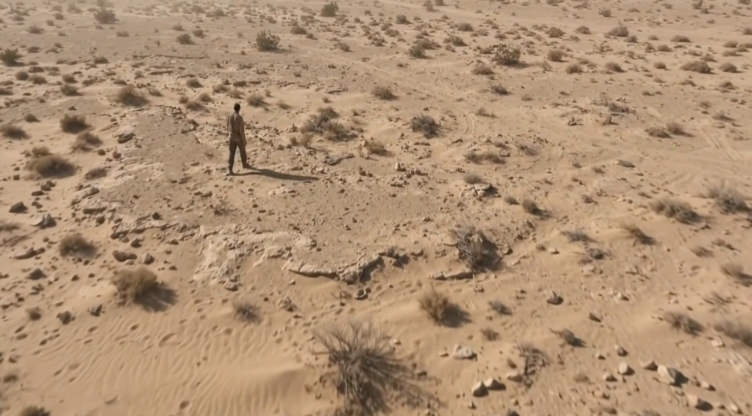
\includegraphics[width=1.12cm]{figures/grok_desert_video.png} &
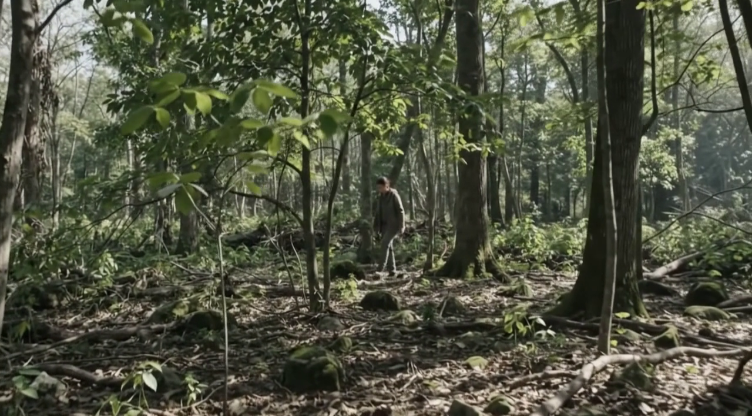
\includegraphics[width=1.12cm]{figures/grok_forest_video.png} &
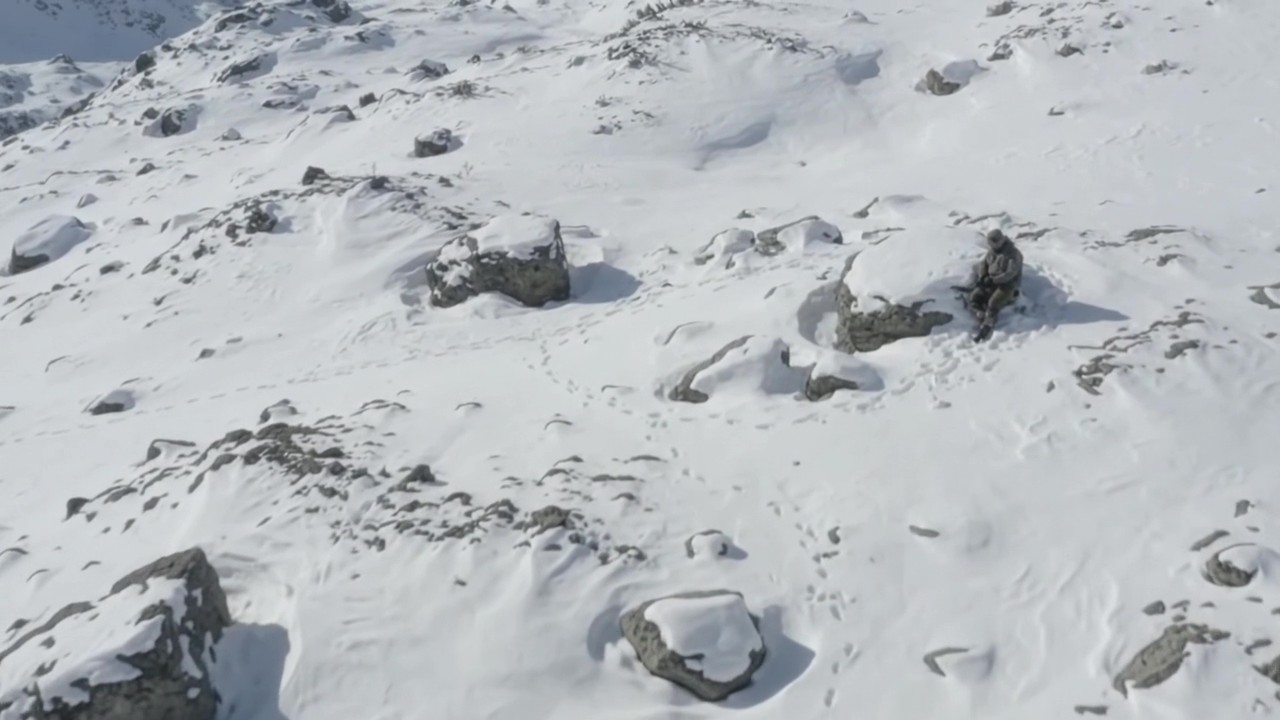
\includegraphics[width=1.12cm]{figures/snow_rgb_video.jpg} \\
{\tiny\bfseries Desert RGB} & {\tiny\bfseries Forest RGB} & {\tiny\bfseries Snow RGB}
\end{tabular}
};
\node[above=3pt of grok_videos, ttl, text=black] (lbl_gv) {16:9 RGB Videos};
\node[below=2pt of grok_videos, font=\fontsize{5.3pt}{6.4pt}\selectfont\bfseries, text=black] (sub_gv) {752$\times$416 @ 24 FPS};

\draw[bluearrow] (grok_rgb.east) -- (grok_videos.west);

\node[videobox] (rgb_videos) at (2.6, 4.85) {
\begin{tabular}{@{}c@{\hspace{3pt}}c@{\hspace{3pt}}c@{}}
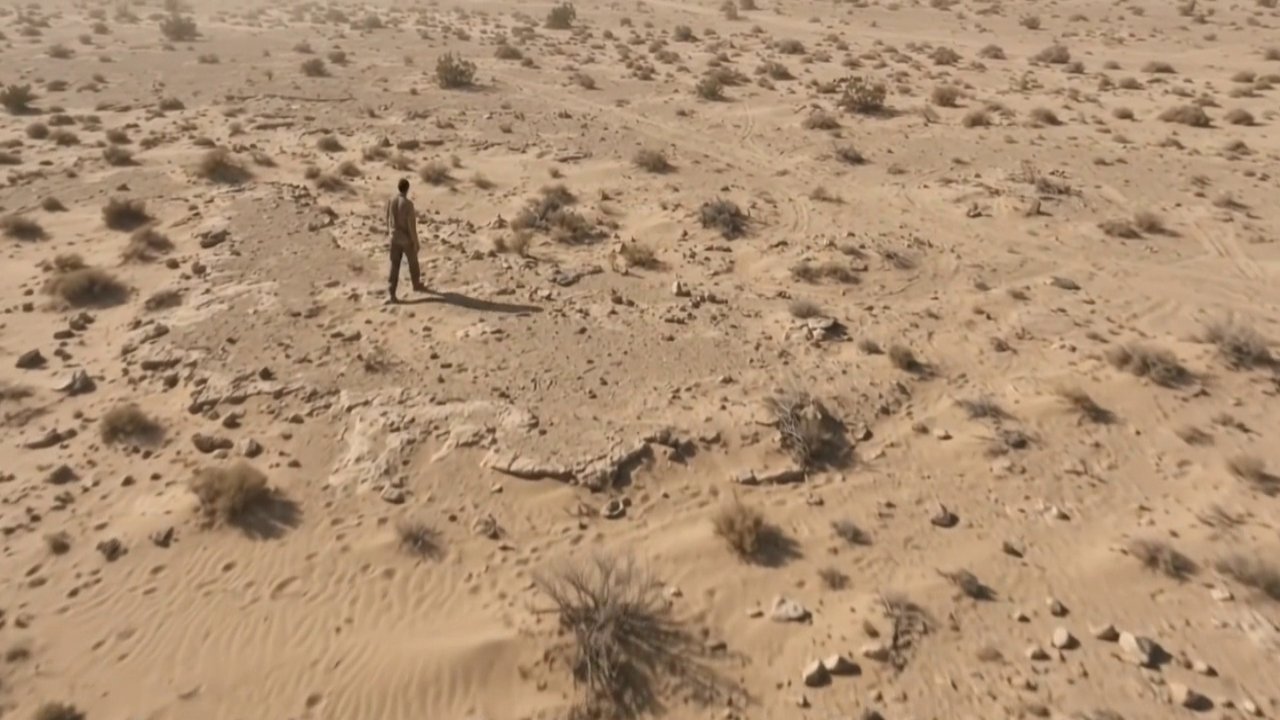
\includegraphics[width=1.12cm]{figures/desert_rgb_video.png} &
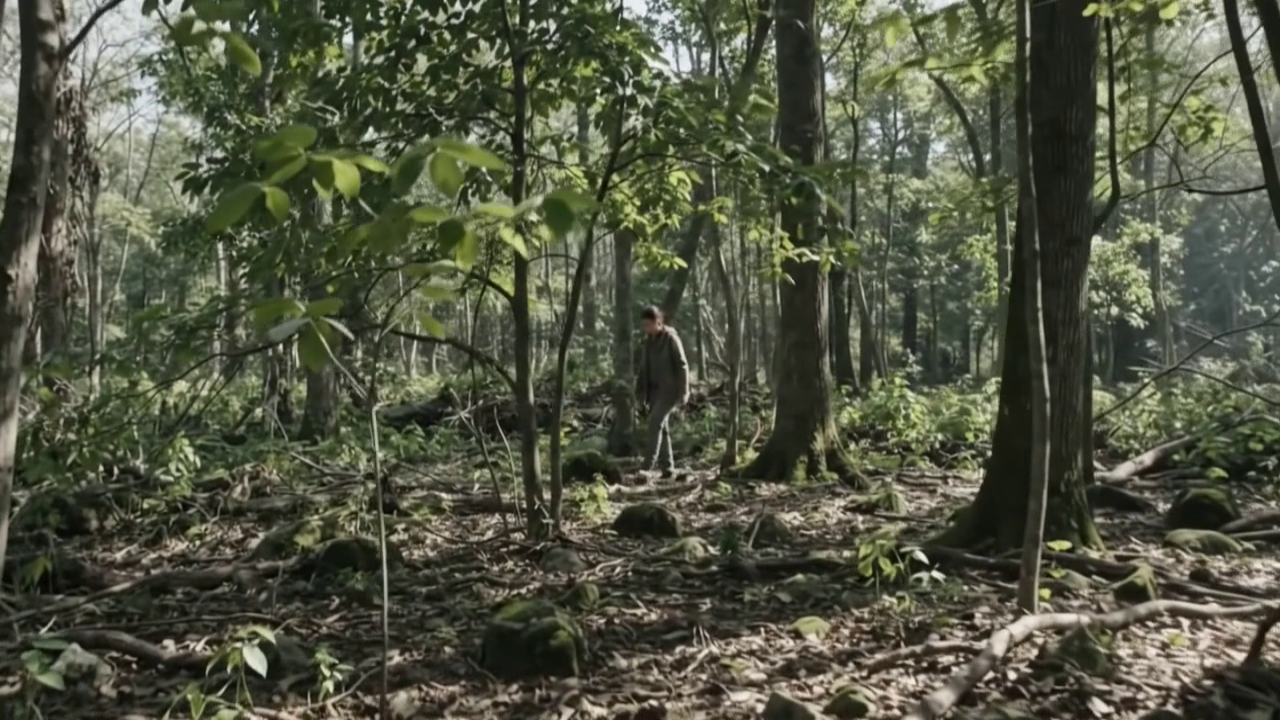
\includegraphics[width=1.12cm]{figures/forest_rgb_video.png} &
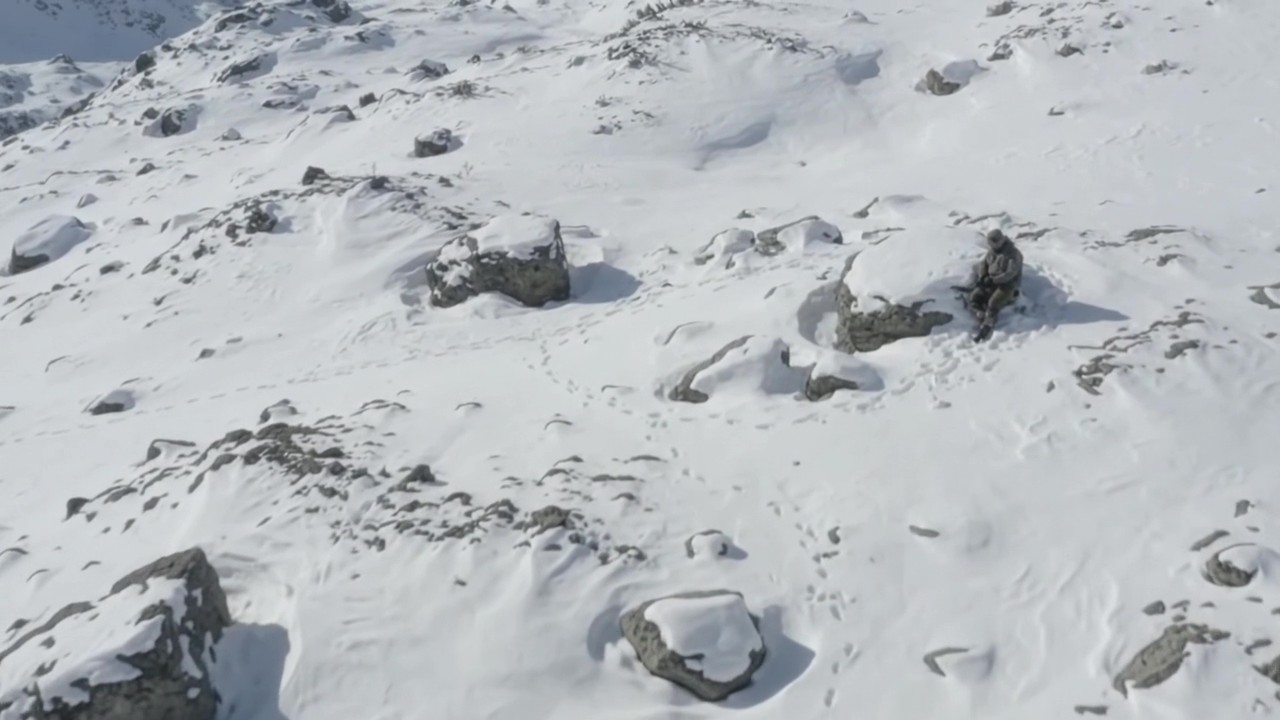
\includegraphics[width=1.12cm]{figures/snow_rgb_video.jpg} \\
{\tiny\bfseries Desert RGB} & {\tiny\bfseries Forest RGB} & {\tiny\bfseries Snow RGB}
\end{tabular}
};
\node[above=3pt of rgb_videos, ttl, text=black] (lbl_v1) {16:9 RGB Videos};
\node[below=2pt of rgb_videos, font=\fontsize{5.3pt}{6.4pt}\selectfont\bfseries, text=black] (sub_v1) {1280$\times$720 @ 24 FPS};

\draw[bluearrow] (gemini_rgb.east) -- (rgb_videos.west);

% 4. Resolution Upscale
\node[box, fill=blue!8, draw=blue!70!black, thick, font=\fontsize{5.6pt}{6.6pt}\selectfont, text width=2.1cm, align=center, minimum height=1.05cm] (upscale_box) at (6.6, 7.35) {
\textbf{Upscale to}\\[1pt]
\textbf{1280$\times$720}\\[2pt]
{\tiny Spatial Scaling}
};
\node[above=3pt of upscale_box, ttl, text=blue!80!black] (lbl_up) {Resolution Upscale};

\draw[bluearrow] (grok_videos.east) -- (upscale_box.west);

% 5. Melo Thermal Stylizing
\node[box, fill=orange!10, draw=orange!80!black, thick, font=\fontsize{5.6pt}{6.6pt}\selectfont, text width=2.6cm, align=center, minimum height=1.15cm] (melo_th) at (10.0, 6.0) {
\textbf{256-Level Color LUT}\\[2pt]
{\scriptsize Grayscale-to-TIR Remap}\\[1pt]
{\tiny Synthetic TIR Emulation}
};
\node[above=4pt of melo_th, ttl, text=orange!80!black] (lbl_melo) {Pseudo-Thermal Transfer};
\node[below=3pt of melo_th, font=\fontsize{5.3pt}{6.4pt}\selectfont\bfseries, text=black] (sub_melo) {LUT Color Mapping};

\draw[orangearrow] (upscale_box.east) -- ([yshift=5pt]melo_th.west);
\draw[orangearrow] (rgb_videos.east) -- ([yshift=-5pt]melo_th.west);

% 6. 16:9 Thermal Videos
\node[videobox] (th_videos) at (14.5, 6.0) {
\begin{tabular}{@{}c@{\hspace{3pt}}c@{\hspace{3pt}}c@{}}
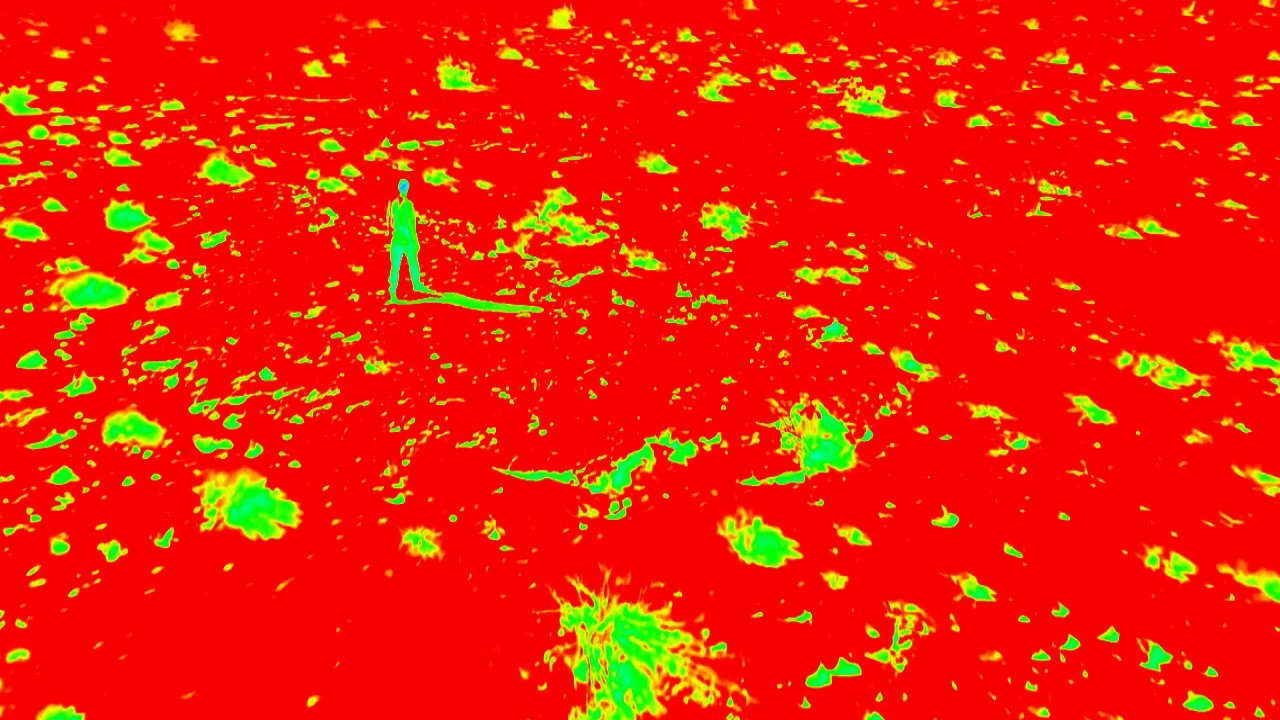
\includegraphics[width=1.12cm]{figures/desert_th_video.png} &
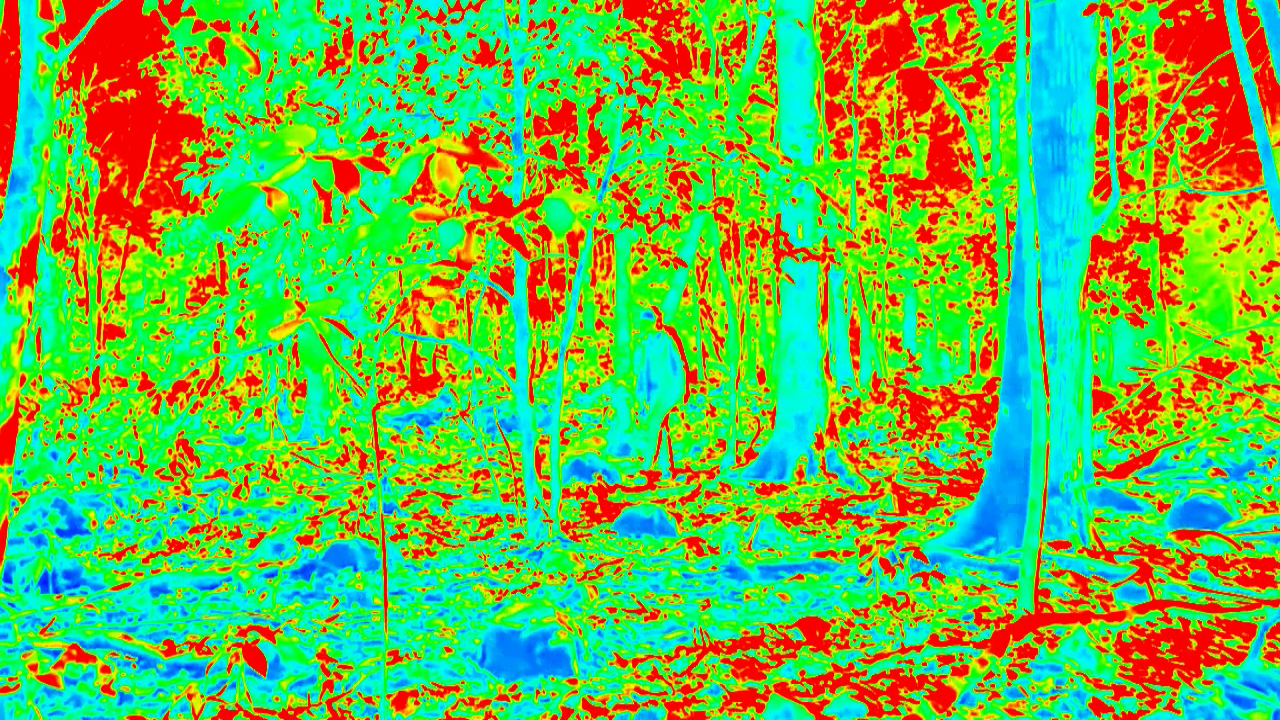
\includegraphics[width=1.12cm]{figures/forest_th_video.png} &

\includegraphics[width=1.12cm]{figures/snow_th_video.jpg.png} \\
{\tiny\bfseries Desert TIR} & {\tiny\bfseries Forest TIR} & {\tiny\bfseries Snow TIR}
\end{tabular}
};
\node[above=4pt of th_videos, ttl, text=black] (lbl_v2) {16:9 Thermal Videos};
\node[below=2pt of th_videos, font=\fontsize{5.3pt}{6.4pt}\selectfont\bfseries, text=black] (sub_v2) {1280$\times$720 @ 24 FPS};

\draw[orangearrow] (melo_th.east) -- (th_videos.west);

% 7. Crop 640x640
\node[videobox] (crops) at (18.5, 6.0) {
\begin{tabular}{@{}c@{\hspace{3pt}}c@{}}
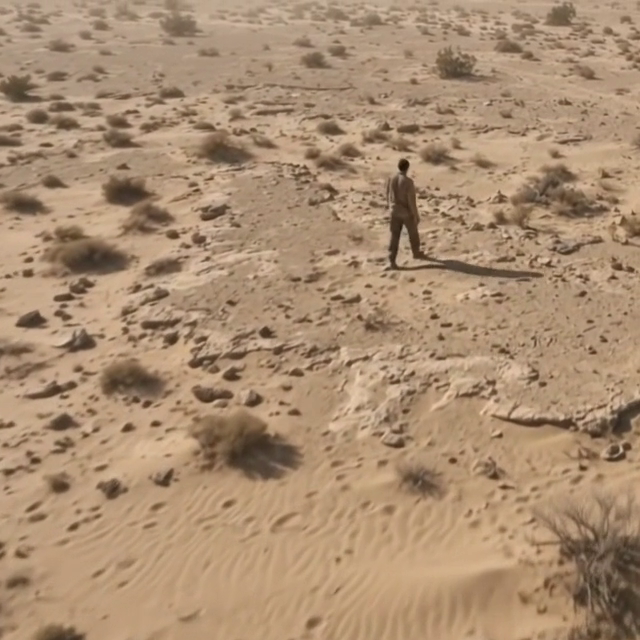
\includegraphics[width=0.83cm]{figures/crop_640_left_video.png} &
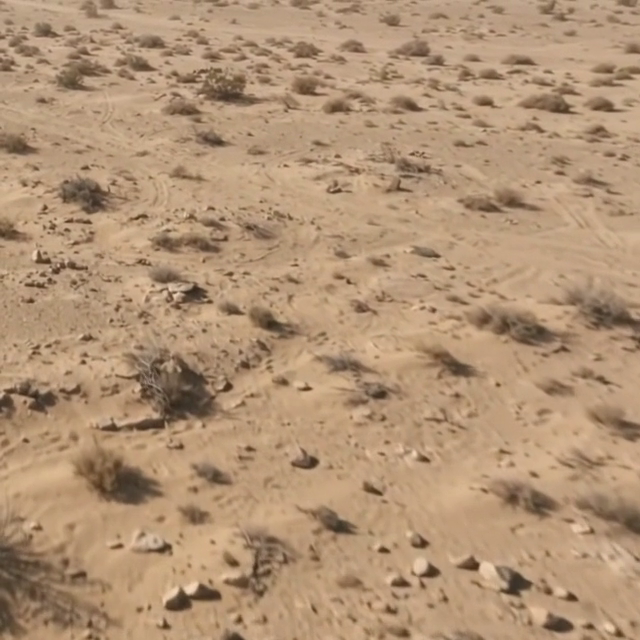
\includegraphics[width=0.83cm]{figures/crop_640_right_video.png} \\
{\tiny\bfseries Left ($x=0$)} & {\tiny\bfseries Right ($x=640$)}
\end{tabular}
};
\node[above=4pt of crops, ttl, text=purple!80!black] (lbl_c) {Crop 640$\times$640 (2 Videos)};
\node[below=2pt of crops, font=\fontsize{5.3pt}{6.4pt}\selectfont\bfseries, text=black] (sub_c) {Cropped Videos (24 FPS)};

\draw[purplearrow] (th_videos) -- (crops);

% 8. Label Studio
\node[iconbox] (label_studio) at (21.6, 6.0) {

\includegraphics[height=0.76cm]{figures/icon_label_studio.png}
};
\node[above=4pt of label_studio, ttl, text=red!80!black] (lbl_ls) {Label Studio};
\node[below=2pt of label_studio, font=\fontsize{5.3pt}{6.4pt}\selectfont\bfseries, text=black] (sub_ls) {Video Annotation};

\draw[purplearrow] (crops) -- (label_studio);

% 9. Video to Frame
\node[stepbox, text width=1.95cm, inner xsep=3pt, minimum height=1.15cm] (v2f) at (24.2, 6.0) {
\textbf{Video to Frame}\\[2pt]
{\scriptsize Full-Rate Stream}\\[-1pt]
{\scriptsize (24~Hz Sampling)}
};
\node[below=2pt of v2f, font=\fontsize{5.3pt}{6.4pt}\selectfont\bfseries, text=black] (sub_v2f) {Frame Extraction};

\draw[greenarrow] (label_studio) -- (v2f);

% 10. Annotated Frames — NO Snow RGB
\node[framebox] (annotated_frames) at (28.0, 6.0) {
\begin{tabular}{@{}c@{\hspace{3pt}}c@{\hspace{3pt}}c@{}}
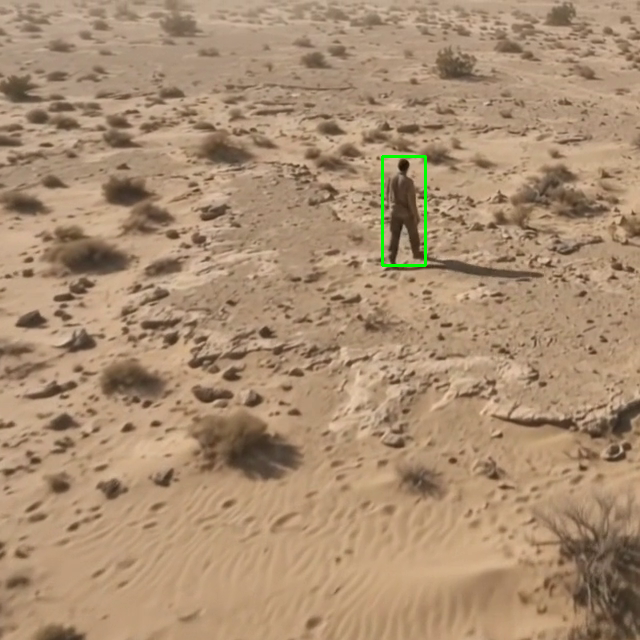
\includegraphics[width=0.82cm]{figures/desert_rgb_annotated.png} &
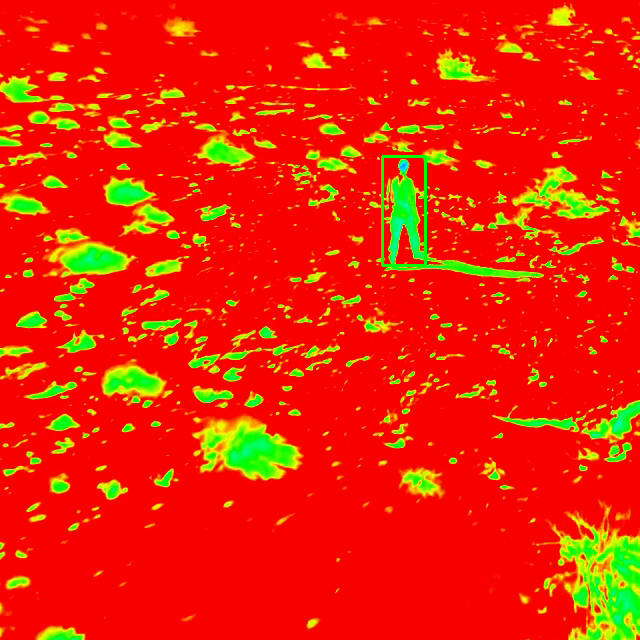
\includegraphics[width=0.82cm]{figures/desert_th_annotated.png} &
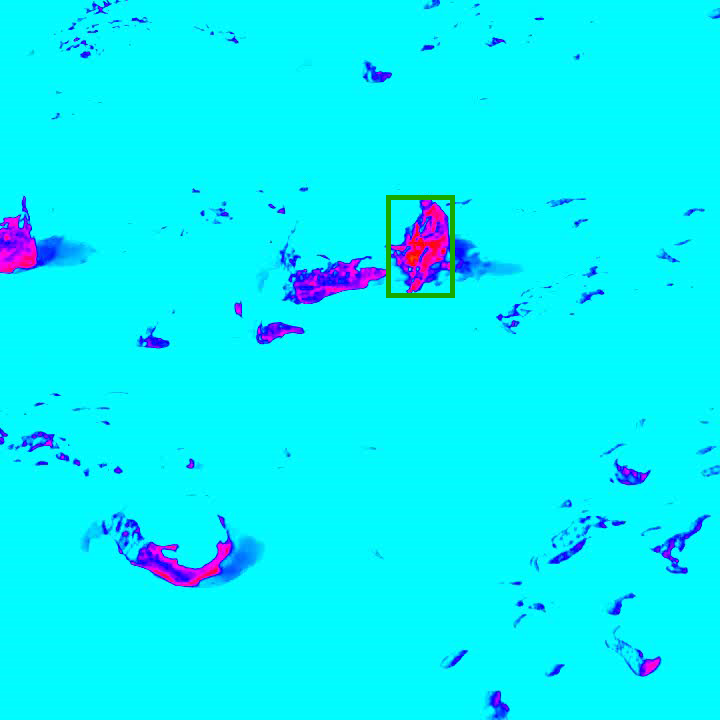
\includegraphics[width=0.82cm]{figures/snow_th_annotated.png} \\
{\tiny\bfseries RGB Frame} & {\tiny\bfseries Thermal Frame} & {\tiny\bfseries Snow TIR}
\end{tabular}
};
\node[above=4pt of annotated_frames, ttl, text=teal!80!black] (lbl_af) {Annotated Frames};
\node[below=2pt of annotated_frames, font=\fontsize{5.3pt}{6.4pt}\selectfont\bfseries, text=black] (sub_af) {Dataset Frames};

\draw[greenarrow] (v2f) -- (annotated_frames);

% =========================================================================
% MIDDLE SECTION: DATASET BANNER
% =========================================================================

\node[draw=purple!70, fill=purple!6, rounded corners=4pt, thick, font=\fontsize{5.8pt}{7.0pt}\selectfont, text=black, inner ysep=4pt, inner xsep=10pt, align=center] (dataset_banner) at (13.5, 3.65) {
\textbf{\textcolor{purple!90!black}{Benchmark Corpus and Sequence Partitioning (Option B)}}\\[2pt]
Parent-Video Grouped Split (44/22/24 tiles $\approx$ 49\%/24\%/27\%) $|$ Co-Located Left and Right Tiles\\
240 Frames/Episode at 24~Hz ($0 \to 239$ Sequential) $|$ Seed 0 Shuffled with Anti-Adjacency
};

\draw[thick, draw=purple!80, ->] (annotated_frames.east) -- ++(0.5, 0) |- (dataset_banner.east);

% =========================================================================
% BOTTOM SECTION: DETECTION, FUSION & POST-PROCESSING
% =========================================================================

\node[box, fill=purple!10, draw=purple!75, thick, font=\fontsize{5.2pt}{6.4pt}\selectfont, text width=1.9cm, align=center] (split_box) at (-1.0, -0.7) {
\textbf{Corpus Split}\\[1pt]
\textbf{Dispatch}\\[2pt]
{\scriptsize Option B Partition}\\[1pt]
{\tiny Shuffled Episodes}
};

\coordinate (split_bus) at (-3.2, 3.65);
\draw[thick, draw=purple!80] (dataset_banner.west) -- node[midway, below=3.5pt, sig, text=purple!90!black] {Curated Dataset Stream} (split_bus);
\draw[arrow, draw=purple!80, thick] (split_bus) |- (split_box.west);

% Detectors
\node[detector] (yolo_rgb) at (3.2, 0.6) {\textbf{RGB Detector}\\[1pt]YOLO11n\\[1pt]{\scriptsize 640$\times$640, 2.6M}\\[-1pt]{\scriptsize Batch: 16, FP32}};
\node[detector] (yolo_tir) at (3.2, -2.0) {\textbf{Thermal Detector}\\[1pt]YOLO11n\\[1pt]{\scriptsize 640$\times$640, 2.6M}\\[-1pt]{\scriptsize Batch: 16, FP32}};

\draw[arrow, blue!70!black, thick] (split_box.north east) to[out=20, in=180] node[pos=0.45, above=4pt, sig] {RGB Input} (yolo_rgb.west);
\draw[arrow, orange!70!black, thick] (split_box.south east) to[out=-20, in=180] node[pos=0.45, below=8pt, sig] {Thermal Input} (yolo_tir.west);

% Late Decision Fusion
\node[fusion] (fusion) at (7.2, -0.7) {
\textbf{Late Decision Fusion}\\[2pt]
Confidence Max Gate\\[2pt]
{\scriptsize Soft Disjunctive OR}
};

\draw[arrow, blue!70!black] (yolo_rgb.east) -- node[pos=0.45, above=4pt, sig] {RGB Score} (fusion.north west);
\draw[arrow, orange!70!black] (yolo_tir.east) -- node[pos=0.65, below=4pt, sig] {Thermal Score} (fusion.south west);

% Causal Post-Processing Methods (M1–M6)
\node[method] (m1) at (13.3, 2.15) {\textbf{M1: Raw Baseline}\\[1pt]Direct Score Threshold\\{\tiny (Instantaneous Confidence)}};
\node[method] (m2) at (13.3, 0.85) {\textbf{M2: Moving Average}\\[1pt]Sliding Window Mean\\{\tiny (5-Frame Window, 208 ms)}};
\node[method] (m3) at (13.3, -0.45) {\textbf{M3: Median Filter}\\[1pt]Order-Statistic Median\\{\tiny (Spike Rejection, 5 Frames)}};
\node[method] (m4) at (13.3, -1.75) {\textbf{M4: History Consensus}\\[1pt]Majority Rule Persistence\\{\tiny (At Least 3 of 5 Detections)}};
\node[method] (m5) at (13.3, -3.05) {\textbf{M5: Learned Mamba-SSSM}\\[1pt]Selective State-Space Filter\\{\tiny (Learned Recurrent Dynamics)}};
\node[method] (m6) at (13.3, -4.45) {\textbf{M6: Learned GRU Baseline}\\[1pt]Single-layer GRU ($d_{\mathrm{h}}=16$)\\{\tiny 1\,681 params, 64\,B state}\\[1pt]
{\tiny Edge-compatible; 44 tiles / 5 seeds}};

% Distribution Bus (extended for M6)
\draw[thick, draw=purple!80] (fusion.east) -- (10.2, -0.7) node[midway, above=4pt, sig, text=purple!90!black] {Fused Score};
\draw[thick, draw=purple!80] (10.2, 2.15) -- (10.2, -4.45);
\draw[arrow, draw=purple!80] (10.2, 2.15) -- (m1.west);
\draw[arrow, draw=purple!80] (10.2, 0.85) -- (m2.west);
\draw[arrow, draw=purple!80] (10.2, -0.45) -- (m3.west);
\draw[arrow, draw=purple!80] (10.2, -1.75) -- (m4.west);
\draw[arrow, draw=purple!80] (10.2, -3.05) -- (m5.west);
\draw[arrow, draw=purple!80] (10.2, -4.45) -- (m6.west);

% Collection Bus (extended for M6)
\draw[thick, draw=teal!80] (16.4, 2.15) -- (16.4, -4.45);
\draw[arrow, draw=teal!80] (m1.east) -- (16.4, 2.15);
\draw[arrow, draw=teal!80] (m2.east) -- (16.4, 0.85);
\draw[arrow, draw=teal!80] (m3.east) -- (16.4, -0.45);
\draw[arrow, draw=teal!80] (m4.east) -- (16.4, -1.75);
\draw[arrow, draw=teal!80] (m5.east) -- (16.4, -3.05);
\draw[arrow, draw=teal!80] (m6.east) -- (16.4, -4.45);

% Alert Decision
\node[decision] (alarm) at (18.9, -0.7) {
\textbf{Alert Decision}\\[2pt]
Verification Gate\\[2pt]
{\scriptsize Optimal Threshold $\tau_m^*$}
};
\draw[arrow, draw=teal!80, very thick] (16.4, -0.7) -- (alarm.west);

% KPI + Evaluation
\node[kpi] (kpi_box) at (23.8, 0.75) {
\textbf{Reliable Alert Generation}\\[1pt]
{\scriptsize False Alert Mitigation (FASR)}\\[-1pt]
{\tiny Bounded Decision Latency (208~ms)}
};
\coordinate (alarm_split) at (20.6, -0.7);
\draw[thick, draw=teal!80] (alarm.east) -- (alarm_split);
\draw[arrow, draw=red!70!black, thick, rounded corners=5pt] (alarm_split) |- node[pos=0.72, above=5pt, sig, text=red!80!black] {Alarm Stream} (kpi_box.west);

\node[eval] (eval) at (23.8, -1.95) {
\textbf{Operational Evaluation}\\[2pt]
Detection ($R, P, F_1$)\\[1pt]
False Alert Mitigation\\[1pt]
Decision Delay ($<$208~ms)\\[1pt]
Compute \& Energy Savings
};
\draw[arrow, draw=blue!70!black, thick, rounded corners=5pt] (alarm_split) |- node[pos=0.72, below=5pt, sig, text=blue!80!black] {Alarm Signal} (eval.west);

\end{tikzpicture}}
\caption{MMSAR evaluation framework. Text-to-video models synthesize RGB streams; a 256-level lookup table produces synchronized pseudo-TIR streams. After $2\times$ tiling, annotation, and 24~Hz extraction, parent-video-grouped episodes prevent spatial leakage. Parallel YOLO11n detectors feed the late fusion max gate in Eq.~\eqref{eq:late_fusion} and six causal decision methods ($W=5$, 208~ms window span).}
\label{fig:system_architecture}
\end{figure*}

\section{Introduction}

Autonomous unmanned aerial vehicles (UAVs) provide rapid aerial coverage in wilderness search and rescue (SAR) missions \cite{rudol2008human,silvagni2017multipurpose}. Onboard vision systems must operate under strict Size, Weight, Power, and Cost (SWaP-C) limits, and remote missions often depend on low-bandwidth telemetry \cite{kyrkou2021emergencynet}. In autonomous operations, false alarms trigger costly hover-and-verify maneuvers that drain battery power and can divert attention from an active search.

Wilderness optical sensing suffers from sensor-specific failure modes. Visible red-green-blue (RGB) cameras degrade in dense shadows, heavy foliage, and poor lighting. Real thermal infrared (TIR) cameras can detect body heat regardless of illumination \cite{hwang2015multispectral,jia2021llvip}, though they suffer from thermal crossover when ground temperatures approach human body temperature \cite{portmann2014people}. Calibrated radiometric TIR is impractical to synthesize at scale for this study, so we instead generate a pseudo-TIR channel via a grayscale lookup table applied to synthetic RGB frames. This channel is a luminance-based encoding, not a physical temperature measurement, and we treat it throughout as a second, spectrally-distinct view rather than a radiometric proxy. In practice this means that in desert scenes, sun-heated rocks and skin can both produce high RGB luminance and therefore high pseudo-TIR intensity, loosely analogous to real thermal crossover, while in snow scenes the same encoding makes bright snow appear anomalously ``hot,'' an artifact with no physical counterpart. We combine RGB and pseudo-TIR streams because they fail in different, complementary ways across biomes; this is sufficient to motivate late fusion as a controlled multi-stream stress test even without radiometric realism (Section~V.F).

Small UAVs require compact single-stage detectors such as You Only Look Once (YOLO) \cite{redmon2016you}. We deploy Ultralytics YOLO11n \cite{jocher2024yolo11} (2.6M parameters, 6.5 giga floating-point operations [GFLOPs] at $640 \times 640$) in 32-bit floating-point (FP32) precision. Per-frame detections nonetheless fluctuate due to platform vibration, motion blur, and background clutter, producing brief false alarms in background regions and intermittent dropouts on real targets.

This raises a focused question: given a fixed, already-lightweight multimodal detector, is a learned temporal sequence model needed to turn its noisy scalar confidence stream into a reliable alert, or does simple causal filtering already capture most of the achievable benefit? Frame detections are combined via a late fusion max gate (Section~III) and evaluated using a strictly validation-calibrated decision protocol, described fully in Section~III.C, under which no detector weights, window lengths, or thresholds are tuned on the held-out test split.

This work provides three main contributions: \textit{1) Causal Decision Benchmark and Operating-Point Recommendation:} a controlled evaluation of six causal temporal decision rules (raw thresholding, moving average, median filtering, history consensus, Mamba-SSSM, and GRU) on a fixed multimodal detection stream, yielding two practical operating points (Table~\ref{tab:postprocessing_benchmark}, Fig.~\ref{fig:performance_tradeoff}); \textit{2) Scoped Evidence on Learned Sequence Models:} empirical demonstration that small Mamba-SSSM and GRU models trained on limited data provide no statistically significant alert-reliability gain over simple filters despite $73\times$--$500\times$ higher runtime (Section~V.C); and \textit{3) Multimodal Benchmark and Sensitivity Analysis:} a controlled $3\times 2$ evaluation across desert, forest, and snow biomes under parent-video episodic isolation with recall-weighted threshold sensitivity analysis (Section~V.G).

\section{Related Work}

Multimodal aerial vision combines complementary visible and thermal bands to mitigate environmental extremes, as explored in ground datasets such as KAIST \cite{hwang2015multispectral} and LLVIP \cite{jia2021llvip}. For wilderness SAR, WiSARD \cite{broyles2022wisard} provides multi-viewpoint benchmarks, while Rudol and Doherty \cite{rudol2008human} demonstrated dual-band geolocation from UAVs. Edge UAV deployment remains tightly constrained by SWaP-C limits \cite{silvagni2017multipurpose}, where complex neural ensembles rapidly drain battery reserves \cite{lygouras2019unsupervised}. Single-stage detectors such as YOLO11n \cite{jocher2024yolo11} deliver real-time frame rates, but per-frame detections fluctuate due to motion blur and terrain-driven confidence noise \cite{portmann2014people}, generating false alarms that trigger wasteful hover maneuvers.

Classical sequential decision making addresses temporal fluctuations through statistical tests such as Wald's sequential probability ratio test \cite{wald1945sequential}, radar sliding-window binary integration ($M$-of-$N$) \cite{richards2014fundamentals}, and running median or moving average filters \cite{rabiner1975applications}. More recently, selective state-space models such as Mamba \cite{gu2023mamba} provide linear-time sequence modeling with recurrent state representations. While prior SAR literature emphasizes per-frame bounding box accuracy, the question of whether such learned temporal models are actually needed to convert noisy multimodal scalar confidence streams into reliable mission alerts, under a strict edge latency budget, remains largely uncharacterized. This paper addresses that gap with a head-to-head benchmark on fixed multimodal detector streams.

\section{Methodology}

The pipeline integrates dual-spectrum detection, late fusion, and causal temporal filtering (Fig.~\ref{fig:system_architecture}). Synchronized visible RGB frames $I_{\text{RGB}}[n]$ and pseudo-TIR frames $I_{\text{Thermal}}[n]$ produce per-frame target confidences $c_{\text{RGB}}[n], c_{\text{Thermal}}[n] \in [0.0, 1.0]$. The upstream detectors and late fusion gate remain fixed across all experiments so that only the temporal decision stage varies.

\subsection{Video Ingestion and Real-Time Edge Budget}
Video streams are captured at $f_s = 24\text{ Hz}$, yielding a frame period $T_s \approx 41.7\text{ ms}$. To avoid dropped frames or queue delay, processing must satisfy
\begin{equation}
T_{\text{detect}} + T_{\text{fusion}} + T_{\text{filter}} \le 41.7\text{ ms},
\label{eq:realtime_budget}
\end{equation}
where $T_{\text{detect}} = \max(T_{\text{RGB}}, T_{\text{Thermal}})$ is parallel detection runtime, $T_{\text{fusion}}$ is fusion latency, and $T_{\text{filter}}$ is post-processing latency. We deploy two parallel YOLO11n models \cite{jocher2024yolo11}: \textbf{YOLO11n-RGB} and \textbf{YOLO11n-Thermal}. Frames with no target predictions yield confidence 0.0.

\subsection{Late Fusion Max Gate}
To prevent target dropouts when one sensor is occluded, detector confidences are combined using a late fusion max gate:
\begin{equation}
s[n] = \max\big(c_{\text{RGB}}[n], \, c_{\text{Thermal}}[n]\big) \in [0.0, 1.0].
\label{eq:late_fusion}
\end{equation}
This max gate lets confident detections in either spectrum propagate forward without requiring pixel-level sensor registration.

\subsection{Causal Temporal Post-Processing Methods}
Direct thresholding of the raw fused confidence produces high false-alarm rates from brief clutter spikes. Downstream processing instead buffers the fused stream across a causal sliding window of length $W = 5$ frames: $\mathbf{w}[n] = [s[n-4], \dots, s[n]]$. This window spans $T_{\text{span}} = WT_s = 208.3\text{ ms}$; the maximum causal buffering delay contributed by the filter itself is $T_{\text{buffer}} = (W-1)T_s = 166.7\text{ ms}$, which is distinct from the empirically measured Alert Latency in Section~III.D, since the latter also includes upstream detector confidence ramp-up.

Each method is assigned an optimal baseline decision threshold calibrated on validation sequences $\mathcal{D}_{\text{val}}$ across candidate thresholds from 0.05 to 0.95 (step size 0.02):
\begin{equation}
\tau^* = \arg\max_{\tau \in [0.05, 0.95]} F_1(\tau; \, \mathcal{D}_{\text{val}}).
\label{eq:f1_opt}
\end{equation}
As an operational sensitivity analysis (Section~V.G), we also calibrate thresholds under a recall-weighted regime that prioritizes victim localization over false-alarm suppression. To prevent threshold degeneration into low-confidence background noise when sweeping recall-heavy metrics, the search is bounded by an operational validation precision floor $P(\tau) \ge 0.95$:
\begin{equation}
\tau^*_{F_\beta} = \arg\max_{\substack{\tau \in [0.05, 0.95] \\ P(\tau) \ge 0.95}} F_\beta(\tau),
\label{eq:fbeta}
\end{equation}
where $F_\beta(\tau) = (1+\beta^2)\frac{P(\tau)\,R(\tau)}{\beta^2 P(\tau) + R(\tau)}$, evaluated at $\beta=2$. Equivalently, we evaluate an asymmetric misclassification cost:
\begin{equation}
\tau^*_{C} = \arg\min_{\substack{\tau \in [0.05, 0.95] \\ P(\tau) \ge 0.95}} \big[\, c_{\text{FN}} \cdot \text{FN}(\tau) + c_{\text{FP}} \cdot \text{FP}(\tau) \,\big],
\label{eq:asymcost}
\end{equation}
where $c_{\text{FN}} = 5$ and $c_{\text{FP}} = 1$. \textit{Protocol Lock:} no detector weights, temporal-model parameters, decision thresholds, or window lengths were selected or tuned using the test set.

We evaluate six causal decision strategies: \textbf{M1 (Baseline Raw):} instantaneous thresholding $y[n] = \mathbb{I}(s[n] \ge \tau^*)$ ($O(1)$ time, 0~B buffer); \textbf{M2 (Moving Average):} causal FIR mean $\bar{s}[n] = \frac{1}{W}\sum_{k=0}^{W-1}s[n-k]$ ($O(1)$ time, 20~B buffer); \textbf{M3 (Median Filter):} order-statistic median $\tilde{s}[n] = \text{median}(\mathbf{w}[n])$ rejecting pulses $<3$ frames ($O(W)$ time, 20~B buffer); \textbf{M4 (History Consensus):} 3-of-5 binary voting ($O(W)$ time, 5~B buffer); \textbf{M5 (Learned Mamba-SSSM):} pure-PyTorch SSSM ($d_{\text{model}}=16, d_{\text{state}}=8$, 753 params, 512~B state); and \textbf{M6 (Learned GRU):} recurrent unit ($d_{\text{hidden}}=16$, 1,681 params, 64~B state).
M5 and M6 are deliberately small to remain compatible with edge inference budgets; both are trained on 44 training tiles (9,800 frames per modality) across five seeds, with $\tau^*$ calibrated only on validation sequences. We return to the implications of this scale in Section~V.C.

\subsection{Alert-Level Evaluation Metrics}
To measure operational mission effectiveness, we report four primary alert-level metrics: \textit{1) False Alerts per Minute (FA/min):} rate of false alarm events during non-target periods, $\text{FA/min} = K_{\text{FA}} / T_{\text{flight}}$, where an alarm event is a contiguous run of positive detections ($y[n]=1$). \textit{2) Positive Target Recall (\%):} proportion of ground-truth target tiles for which at least one confirmed alert is produced. \textit{3) Alert Latency (Time-to-Alarm):} elapsed flight time from target entrance in the camera FOV to the first asserted alert, capturing both filter buffering delay and detector ramp-up. \textit{4) False Alarm Suppression Ratio (FASR):} percentage reduction in false alarm frames relative to the raw baseline: $\text{FASR} = 1 - (\text{FP}_{\text{filter}} / \text{FP}_{\text{raw}})$.

\section{Experimental Setup and Dataset}

Wilderness SAR dual-spectrum datasets remain scarce. As summarized in Table~\ref{tab:system_config}, our controlled $3\times 2$ design balances modality and environment across three wilderness biomes: \textit{1) Arid Desert:} rocky terrain, sparse vegetation, and midday lighting under which sun-heated rock surfaces can produce pseudo-TIR intensities comparable to human targets (Section~I); \textit{2) Temperate Forest:} dense canopies, dappled shadows, intermittent foliage occlusions, and wildlife distractors; and \textit{3) Snow-Covered Alpine:} high-albedo snow causing visible glare in RGB and anomalously high pseudo-TIR intensity, an encoding artifact rather than a physical thermal effect (Section~V.F).

Qualitatively, desert video streams exhibit clear visible separation but background crossover artifacts; forest sequences present intermittent tree canopy occlusions in both channels; and snow alpine scenes show high luminance reflection on snowpack.

\begin{table}[!t]
\centering
\caption{Corpus Partitioning and Experimental System Specifications}
\label{tab:system_config}
\resizebox{\columnwidth}{!}{%
\begin{tabular}{ll}
\toprule
\textbf{System Parameter} & \textbf{Design Specification / Value} \\
\midrule
Environments & Arid Desert (30 tiles), Temperate Forest (28 tiles), \\
             & Snow-Covered Alpine (32 tiles) \\
Sensor Modalities & Synchronized visible RGB and pseudo-thermal infrared (TIR) \\
Raw Video Format & $1280 \times 720$ at 24~Hz ($T_s \approx 41.7\text{ ms}$), 10.0~s nominal \\
Dual-Crop Tiling & $2\times$ square tiles ($640 \times 640$, left/right, $y = 40$) \\
Corpus Volume & 90 tiles, 20,364 frames per modality (40,728 total frames; \\
              & 42 positive tiles [5,620 frames], 48 negative distractor tiles [14,744 frames]) \\
Episodic Partition & Option B parent-grouped (realized: 44 train [17 pos, 27 neg], \\
                   & 22 val [12 pos, 10 neg], 24 test [13 pos, 11 neg] tiles per modality) \\
Upstream Detectors & Dual YOLO11n (2.6M params, 6.5 GFLOPs at $640\times 640$, FP32) \\
Training Setup & Batch 16, 60 epochs, SGD cosine schedule ($\text{lr}_0=0.01$) \\
Decision Window & Sliding causal window $W \in \{1, 3, 5, 7\}$ ($W=5$ nominal; 208~ms span) \\
Decision Strategies & Raw (M1), Moving Avg (M2), Median (M3), Consensus (M4), \\
                    & Mamba-SSSM (M5), GRU Baseline (M6) \\
\bottomrule
\end{tabular}%
}
\end{table}

Raw video is captured at $1280 \times 720$ and 24~Hz. A $2\times$ dual-crop extraction preserves ground sampling distance without downsampling small targets, producing disjoint $640 \times 640$ left/right tiles ($y=40$). The corpus contains 30 desert, 28 forest, and 32 snow-alpine tiles (90 per modality; 42 positive and 48 negative), totaling 20,364 frames per modality. Label Studio keyframe interpolation provides ground-truth boxes.

Partitioning is conducted strictly at the parent-video level using parent-video grouped episodic partitioning to prevent spatial or temporal leakage between derived sibling tiles; left and right sibling tiles share a partition. The realized partition allocates 44 training tiles (17 positive, 27 negative; 9,800 frames per modality), 22 validation tiles (12 positive, 10 negative; 4,994 frames per modality), and 24 testing tiles (13 positive, 11 negative; 5,570 frames per modality). In the held-out test split, each biome contributes 8 tiles (desert: 4 positive, 4 negative; forest: 4 positive, 4 negative; snow alpine: 5 positive, 3 negative). Frames remain in exact chronological order to support causal evaluation.

\section{Results and Discussion}

\subsection{Upstream Detection Across Modalities and Biomes}
We first evaluate frame-level detection performance of the two fixed YOLO11n models and the late fusion max gate on the held-out test split under standard thresholding ($\tau = 0.50$). Table~\ref{tab:fusion_comparison} summarizes precision, recall, and F1-score across biomes.

\begin{table}[!t]
\centering
\caption{Frame-Level Upstream Detection Performance and Modality Progression on Held-Out Test Split (Fixed Detectors, Threshold $\tau = 0.50$)}
\label{tab:fusion_comparison}
\resizebox{\columnwidth}{!}{%
\begin{tabular}{lccc}
\toprule
\textbf{Sensing Configuration / Environment} & \textbf{Precision} & \textbf{Recall} & \textbf{F1-Score} \\
\midrule
\multicolumn{4}{l}{\textit{Arid Desert Biome}} \\
\quad YOLO11n-RGB          & 0.970 & 0.868 & 0.916 \\
\quad YOLO11n-Thermal      & \textbf{0.997} & 0.851 & 0.918 \\
\quad Late Fusion Max Gate & 0.970 & \textbf{0.942} & \textbf{0.956} \\
\midrule
\multicolumn{4}{l}{\textit{Temperate Forest Biome}} \\
\quad YOLO11n-RGB          & \textbf{0.922} & 0.444 & 0.599 \\
\quad YOLO11n-Thermal      & 0.915 & 0.318 & 0.471 \\
\quad Late Fusion Max Gate & 0.907 & \textbf{0.521} & \textbf{0.662} \\
\midrule
\multicolumn{4}{l}{\textit{Snow/Alpine Biome}} \\
\quad YOLO11n-RGB          & \textbf{0.997} & 0.523 & 0.686 \\
\quad YOLO11n-Thermal      & 0.952 & 0.206 & 0.338 \\
\quad Late Fusion Max Gate & 0.978 & \textbf{0.537} & \textbf{0.693} \\
\midrule
\multicolumn{4}{l}{\textit{Modality Progression (Overall Test Set, 5,570 frames)}} \\
YOLO11n-RGB (Raw, $\tau=0.50$)                    & 0.967 & 0.637 & 0.768 \\
YOLO11n-Thermal (Raw, $\tau=0.50$)                & 0.975 & 0.492 & 0.654 \\
Late Fusion Max Gate (Raw, $\tau=0.50$)           & 0.958 & \textbf{0.693} & \textbf{0.804} \\
Late Fusion Max + Moving Avg ($W=5, \tau^*=0.57$) & \textbf{0.978} & 0.650 & 0.781 \\
\bottomrule
\multicolumn{4}{l}{\footnotesize Bold indicates best result per group. Max-pooling maximizes recall} \\
\multicolumn{4}{l}{\footnotesize while temporal smoothing maximizes precision by rejecting noise spikes.}
\end{tabular}%
}
\end{table}

The upstream modalities show distinct failure modes across environments: visible RGB provides sharp localization under open sunlight but loses recall under dense forest canopy shadows (44.4\%); the pseudo-TIR stream is attenuated by thick foliage (forest recall 31.8\%, though 91.5\% precision on visible patches) and produces false positives over sun-heated desert rock. Combining both streams via the late fusion max gate (Eq.~\eqref{eq:late_fusion}) mitigates these unimodal dropouts, raising forest frame-level recall to 52.1\% ($+7.7\%$ over RGB, $+20.3\%$ over thermal) and reaching 94.2\% recall in desert. Because max-pooling forwards the highest confidence score, it also propagates isolated noise spikes into downstream decision buffers, producing false alarms over negative distractor scenes. Multi-seed detector evaluation (seeds 0, 42, 1234) confirmed stable upstream convergence ($\text{mAP}_{50} = 0.985 \pm 0.008$, $\text{mAP}_{50-95} = 0.518 \pm 0.017$), motivating the temporal filtering stage below.

\begin{figure}[!t]
\centering
\resizebox{0.80\columnwidth}{!}{% Requires in preamble:
% \usepackage{pgfplots}
% \pgfplotsset{compat=1.18}
% \usetikzlibrary{arrows.meta}

\definecolor{cblue}{RGB}{0, 85, 150}
\definecolor{cvermilion}{RGB}{215, 85, 0}
\definecolor{cpurple}{RGB}{115, 50, 130}

\begin{tikzpicture}
  \pgfplotsset{
    scale only axis,
    width=0.72\columnwidth, % Sized to reserve gutter space for right-side threshold labels
    xmin=0,
    xmax=60,
    tick label style={font=\tiny},
    axis line style={semithick, black!75},
    grid style={dotted, black!18, line width=0.5pt},
  }
%
  % -------------------------------------------------------------
  % TOP PANEL: Fused Confidence & Filter Responses
  % -------------------------------------------------------------
  \begin{axis}[
    name=top_axis,
    clip=false, % Allows labels at x=60 to render outside the plot frame
    title={\small\textbf{Temporal Confidence Trace \& Decision Filtering}},
    title style={yshift=2pt},
    height=2.8cm,
    ymin=0,
    ymax=1.18,
    ytick={0.0, 0.5, 1.0},
    ymajorgrids=true,
    ylabel={Confidence $s[n]$},
    ylabel style={font=\scriptsize\bfseries},
    xtick={0, 10, 20, 30, 40, 50, 60},
    xticklabels=\empty,
    axis x line*=bottom,
    axis y line*=left,
  ]
    % Background Intervals
    \fill[black!8] (axis cs:16, 0) rectangle (axis cs:20, 1.18);
    \node[font=\tiny\bfseries, text=black!50, anchor=north] at (axis cs:18, 1.15) {Clutter};

    \fill[black!4] (axis cs:32, 0) rectangle (axis cs:60, 1.18);
    \node[font=\tiny\bfseries, text=black!50, anchor=north] at (axis cs:46, 1.15) {Target Event};

    % Threshold Lines (Labels placed directly to the right of each dashed line)
    \draw[dash pattern=on 3pt off 2pt, draw=cvermilion!85!black, line width=0.7pt] 
      (axis cs:0, 0.57) -- (axis cs:60, 0.57)
      node[right=2pt, font=\tiny\bfseries, text=cvermilion!95!black] {$\tau_{\text{MA}}^* = 0.57$};

    \draw[dashed, draw=black!50, line width=0.6pt] 
      (axis cs:0, 0.43) -- (axis cs:60, 0.43)
      node[right=2pt, font=\tiny\bfseries, text=black!70] {$\tau_{\text{raw}}^* = 0.43$};

    % Trace 1: Fused raw confidence s[n]
    \addplot[
      color=cblue,
      very thick,
      solid,
      mark=*,
      mark repeat=3,
      mark options={scale=0.75, fill=cblue}
    ] coordinates {
      (0, 0.05)  (2, 0.04)  (4, 0.06)  (6, 0.04)  (8, 0.05)
      (10, 0.04) (12, 0.06) (14, 0.05) (16, 0.07) (17, 0.15)
      (18, 0.82) (19, 0.18) (20, 0.06) (22, 0.04) (24, 0.05)
      (26, 0.05) (28, 0.06) (30, 0.07) (31, 0.18) (32, 0.78)
      (34, 0.85) (36, 0.81) (38, 0.88) (40, 0.84) (42, 0.91)
      (44, 0.86) (46, 0.93) (48, 0.89) (50, 0.94) (52, 0.88)
      (54, 0.91) (56, 0.93) (58, 0.89) (60, 0.91)
    };

    % Trace 2: Moving average s_MA[n]
    \addplot[
      color=cvermilion,
      very thick,
      dashed,
      mark=square*,
      mark repeat=3,
      mark options={scale=0.75, fill=cvermilion, solid}
    ] coordinates {
      (0, 0.05)  (8, 0.05)  (14, 0.05) (17, 0.06) (18, 0.21)
      (19, 0.22) (20, 0.23) (21, 0.22) (22, 0.05) (30, 0.06)
      (32, 0.20) (33, 0.38) (34, 0.68) (36, 0.83) (38, 0.84)
      (40, 0.86) (42, 0.88) (46, 0.90) (50, 0.91) (54, 0.91)
      (60, 0.91)
    };
  \end{axis}
%
  % -------------------------------------------------------------
  % BOTTOM PANEL: Alert Waveforms with Expanded Row Padding
  % -------------------------------------------------------------
  \begin{axis}[
    name=bottom_axis,
    at=(top_axis.below south west),
    anchor=above north west,
    yshift=-0.32cm,
    height=3.8cm,
    ymin=-0.2,
    ymax=3.9,
    ytick={0.5, 1.8, 3.1},
    yticklabels={%
      {\bfseries M5 (Mamba)},
      {\bfseries M2 (MA)},
      {\bfseries M1 (Raw)}%
    },
    ylabel={Alert Output},
    ylabel style={font=\scriptsize\bfseries},
    yticklabel style={font=\tiny},
    ymajorgrids=false,
    xmajorgrids=true,
    xtick={0, 10, 20, 30, 40, 50, 60},
    xlabel={Video Frame Index $n$},
    xlabel style={font=\scriptsize\bfseries},
    axis x line*=bottom,
    axis y line*=left,
  ]
    % Aligned Intervals
    \fill[black!8] (axis cs:16, -0.2) rectangle (axis cs:20, 3.9);
    \fill[black!4] (axis cs:32, -0.2) rectangle (axis cs:60, 3.9);

    % Baseline Reference Rails (0-state)
    \draw[black!15, line width=0.5pt] (axis cs:0, 2.8) -- (axis cs:60, 2.8);
    \draw[black!15, line width=0.5pt] (axis cs:0, 1.5) -- (axis cs:60, 1.5);
    \draw[black!15, line width=0.5pt] (axis cs:0, 0.2) -- (axis cs:60, 0.2);

    % M1 (Raw): Spurious pulse at frame 18; onset at frame 31.5
    \addplot[color=cblue, very thick, const plot] coordinates {
      (0, 2.8) (17.5, 3.4) (18.5, 2.8) (31.5, 3.4) (60, 3.4)
    };

    % M2 (MA): Suppressed spike; onset at frame 33.5
    \addplot[color=cvermilion, very thick, dashed, const plot] coordinates {
      (0, 1.5) (33.5, 2.1) (60, 2.1)
    };

    % M5 (Mamba): Suppressed spike; onset at frame 32.5
    \addplot[color=cpurple, very thick, dashdotted, const plot] coordinates {
      (0, 0.2) (32.5, 0.8) (60, 0.8)
    };

    % Clean Latency Measurement
    \draw[dotted, black!40, semithick] (axis cs:31.5, 2.1) -- (axis cs:31.5, 2.55);
    \draw[dotted, black!40, semithick] (axis cs:33.5, 2.1) -- (axis cs:33.5, 2.55);
    \draw[|<->|, semithick, black!75] (axis cs:31.5, 2.45) -- (axis cs:33.5, 2.45);
    \node[anchor=west, font=\tiny\bfseries, text=black!75] at (axis cs:34.0, 2.45) {$\Delta t = 2$};
  \end{axis}
%
  % -------------------------------------------------------------
  % COLOR LEGEND: Centered Below the Bottom X-Axis
  % -------------------------------------------------------------
  \node[
    anchor=north,
    yshift=-0.72cm,
    draw=black!25,
    fill=white,
    rounded corners=2pt,
    font=\tiny,
    inner sep=3.5pt
  ] at (bottom_axis.south) {
    \textcolor{cblue}{\textbf{--$\bullet$--} Fused $s[n]$ (M1)} \hspace{1.4em}
    \textcolor{cvermilion}{\textbf{- -$\blacksquare$- -} Moving Avg $\tilde{s}[n]$ (M2)} \hspace{1.4em}
    \textcolor{cpurple}{\textbf{- $\cdot$ - $\blacktriangle$ - $\cdot$ -} Mamba (M5)}
  };
\end{tikzpicture}}
\caption{Temporal sequence trace: (top) fused confidence $s[n]$ with clutter spike at frame 18 and target event from frame 32; (bottom) causal decisions for M1 (spurious alert), M2 (spike suppressed), and M5.}
\label{fig:real_temporal_sequence}
\end{figure}

\begin{table*}[t]
\centering
\caption{Comparative Benchmark of Causal Temporal Decision Methods on Held-Out Test Sequences ($W = 5$ frames / 208 ms span at 24 Hz)}
\label{tab:postprocessing_benchmark}
\resizebox{\textwidth}{!}{%
\begin{tabular}{lcccccc}
\toprule
\textbf{Decision Method} & \textbf{Val $\tau^*$} & \textbf{Alert Recall (\%)} & \textbf{Frame $F_1$-Score [95\% CI]} & \textbf{False Alerts / min} & \textbf{Alert Latency (Time-to-Alarm)} & \textbf{Filter Runtime / Frame} \\
\midrule
M1: Baseline Raw Thresholding          & 0.43 & \textbf{92.3\% (12/13)} & 0.813 [0.776, 0.847]          & 9.0                         & \textbf{188.9 ms (4.5 frames)}  & \textbf{0.02 $\mu$s ($O(1)$, 0 B state)} \\
M2: Five-Frame Moving Average          & 0.57 & 84.6\% (11/13)          & 0.781 [0.738, 0.822]          & 2.1$^\dagger$               & 592.3 ms (14.2 frames)          & 0.30 $\mu$s ($O(1)$, 20 B state) \\
M3: Five-Frame Median Filter           & 0.49 & \textbf{92.3\% (12/13)} & 0.805 [0.767, 0.841]          & 3.6                         & 291.7 ms (7.0 frames)           & 0.42 $\mu$s ($O(W)$, 20 B state) \\
M4: Five-Frame History Consensus       & 0.49 & \textbf{92.3\% (12/13)} & 0.802 [0.764, 0.838]          & 3.6                         & 313.9 ms (7.5 frames)           & 0.63 $\mu$s ($O(W)$, 5 B state) \\
M5: Learned Mamba-SSSM (5 seeds)       & 0.73 & 87.7\% $\pm$ 4.2\%      & 0.717 $\pm$ 0.040 [0.672, 0.758] & \textbf{1.7 $\pm$ 0.6}     & 587.5 ms (14.1 frames)          & 150.59 $\mu$s ($O(d_{\text{model}}d_{\text{state}})$, 512 B) \\
M6: Learned GRU Baseline (5 seeds)     & 0.50 & 86.2\% $\pm$ 3.4\%      & \textbf{0.822 $\pm$ 0.007 [0.785, 0.856]} & 3.7 $\pm$ 0.3  & 577.3 ms (13.9 frames)          & 21.80 $\mu$s ($O(d_{\text{hidden}}^2)$, 64 B) \\
\bottomrule
\multicolumn{7}{l}{\footnotesize Bold indicates best metric in column. $^\dagger$M2 achieves the lowest FA/min among non-learned methods; difference vs. M5 is not statistically significant ($p = 0.4922$).}
\end{tabular}%
}
\end{table*}

\subsection{Two Operating Points: False-Alert Suppression versus Recall Preservation}
Across the held-out test split, causal filtering establishes two practical operating points rather than a single winner (Table~\ref{tab:postprocessing_benchmark}, Fig.~\ref{fig:performance_tradeoff}). If false-alert suppression is the priority, the five-frame moving average (M2) is the strongest non-learned option: false alerts fall 77\%, from 9.0 to 2.1 FA/min (65.3\% FASR, false-positive frames $75\to26$), with paired Wilcoxon tests confirming fewer false-positive frames ($W=2.0$, $p=0.0056$) and false-alert events ($W=2.0$, $p=0.0087$) than M1. This comes at reduced recall (84.6\%, 11/13 tiles) and longer alert latency (592.3~ms).

If recall preservation is the priority, which matters in SAR settings where a missed target is typically costlier than an extra verification maneuver, the five-frame median filter (M3) and 3-of-5 history consensus (M4) retain the full baseline recall of raw thresholding (92.3\%, 12/13 tiles) while still cutting false alerts by 60\% (3.6 FA/min, 32.0\% FASR) and responding roughly twice as fast as M2 (291.7~ms and 313.9~ms, respectively). For $W=5$, M3 and M4 are equivalent after the initial two-frame fill-up (14 false alerts, 51 FP frames each); M3 is preferable on cost, since it needs no running detection count. M2 yields significantly fewer FP frames ($W=0.0$, $p=0.0047$) and alert events ($W=0.0$, $p=0.0143$) than M3, quantifying the smoothing-sensitivity trade-off directly.

Which operating point is preferable is a mission-design choice rather than a property of the filters alone, and we report both instead of selecting one as globally optimal.

\begin{figure}[!t]
\centering
\resizebox{0.98\columnwidth}{!}{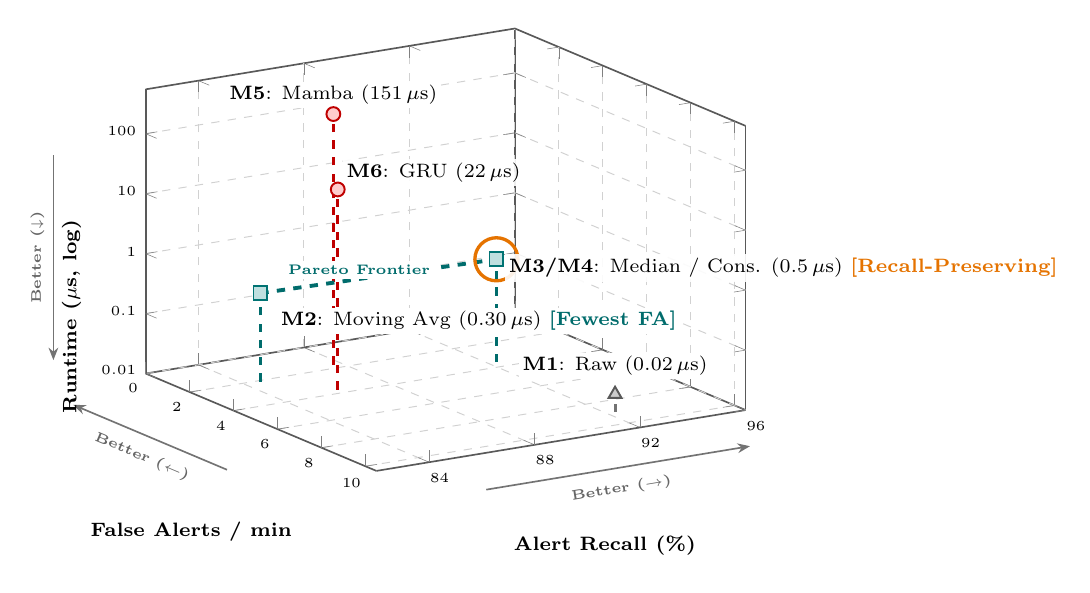
\begin{tikzpicture}
\begin{axis}[
  width=9.2cm,
  height=7.2cm,
  view={58}{22},
  xmin=0, xmax=10.5,
  ymin=82, ymax=96,
  zmode=log,
  zmin=0.01, zmax=550,
  zminorticks=false,
  xtick={0, 2, 4, 6, 8, 10},
  ytick={84, 88, 92, 96},
  ztick={0.01, 0.1, 1, 10, 100},
  zticklabels={$0.01$, $0.1$, $1$, $10$, $100$},
  xlabel={\textbf{False Alerts / min}},
  ylabel={\textbf{Alert Recall (\%)}},
zlabel={\textbf{Runtime ($\mu\text{s}$, log)}},
  xlabel style={font=\scriptsize, yshift=-10pt},
  ylabel style={font=\scriptsize, yshift=-14pt},
  zlabel style={font=\scriptsize, xshift=-34pt},
  tick label style={font=\tiny},
  axis line style={semithick, black!65},
  grid=major,
  grid style={line width=0.35pt, draw=black!18, dashed},
  clip=false
]

  % 1. Directional Improvement Arrows
  \draw[-{Stealth[length=4.5pt, width=3.5pt]}, semithick, black!55] 
    (axis cs:8.5, 78.0, 0.01) -- (axis cs:1.5, 78.0, 0.01)
    node[pos=0.5, sloped, below=1.5pt, font=\tiny\bfseries, text=black!60] {Better ($\leftarrow$)};

  \draw[-{Stealth[length=4.5pt, width=3.5pt]}, semithick, black!55, yshift=-4pt] 
    (axis cs:12.5, 84.5, 0.01) -- (axis cs:12.5, 94.5, 0.01)
    node[pos=0.5, sloped, below=1.5pt, font=\tiny\bfseries, text=black!60] {Better ($\rightarrow$)};

  \draw[{Stealth[length=4.5pt, width=3.5pt]}-, semithick, black!55] 
    (axis cs:0, 78.5, 0.03) -- (axis cs:0, 78.5, 80.0)
    node[pos=0.5, sloped, above=2pt, font=\tiny\bfseries, text=black!60, fill=white, inner sep=1pt] {Better ($\downarrow$)};

  % 2. Depth Drop Lines
  \draw[dashed, black!55,     line width=1.1pt] (axis cs:9.0, 92.3, 0.01) -- (axis cs:9.0, 92.3, 0.02);
  \draw[dashed, teal!85!black, line width=1.1pt] (axis cs:2.1, 84.6, 0.01) -- (axis cs:2.1, 84.6, 0.30);
  \draw[dashed, teal!85!black, line width=1.1pt] (axis cs:3.6, 92.3, 0.01) -- (axis cs:3.6, 92.3, 0.52);
  \draw[dashed, red!75!black,  line width=1.1pt] (axis cs:3.7, 86.2, 0.01) -- (axis cs:3.7, 86.2, 21.8);
  \draw[dashed, red!75!black,  line width=1.1pt] (axis cs:1.7, 87.7, 0.01) -- (axis cs:1.7, 87.7, 150.6);

  % 3. Sub-Microsecond Pareto Frontier
  \addplot3[
    color=teal!85!black,
    line width=1.4pt,
    dashed
  ] coordinates {
    (2.1, 84.6, 0.30)
    (3.6, 92.3, 0.52)
  };

  \node[font=\tiny\bfseries, text=teal!85!black, fill=white, inner sep=1.5pt, sloped, above] 
    at (axis cs:2.75, 87.8, 0.38) {Pareto Frontier};

  % 4. Method Markers & Annotations
  \addplot3[
    only marks,
    mark=square*,
    mark size=2.5pt,
    draw=teal!90!black,
    fill=teal!25,
    line width=0.7pt
  ] coordinates {
    (2.1, 84.6, 0.30)
    (3.6, 92.3, 0.52)
  };

  \node[
    draw=orange!90!black,
    line width=1.2pt,
    circle,
    inner sep=5.5pt
  ] at (axis cs:3.6, 92.3, 0.52) {};

  \node[font=\scriptsize, anchor=north west, fill=white, inner sep=1.2pt] 
[xshift=6pt, yshift=15pt] at (axis cs:2.1, 84.6, 0.035) {\textbf{M2}: Moving Avg ($0.30\,\mu\text{s}$) \textbf{\textcolor{teal!85!black}{[Fewest FA]}}};

  \node[font=\scriptsize, anchor=west, fill=white, fill opacity=0.9, text opacity=1, inner sep=1.5pt] 
at (axis cs:3.95, 92.3, 0.42) {\textbf{M3/M4}: Median / Cons. ($0.5\,\mu\text{s}$) \textbf{\textcolor{orange!90!black}{[Recall-Preserving]}}};

  \addplot3[
    only marks,
    mark=*,
    mark size=2.5pt,
    draw=red!75!black,
    fill=red!20,
    line width=0.7pt
  ] coordinates {
    (1.7, 87.7, 150.6)
    (3.7, 86.2, 21.8)
  };

  \node[font=\scriptsize, anchor=south, fill=white, inner sep=1.2pt] 
    at (axis cs:1.7, 87.7, 185.0) {\textbf{M5}: Mamba ($151\,\mu\text{s}$)};

  \node[font=\scriptsize, anchor=south west, fill=white, fill opacity=0.9, text opacity=1, inner sep=1.4pt] 
    at (axis cs:3.9, 86.2, 26.0) {\textbf{M6}: GRU ($22\,\mu\text{s}$)};

  \addplot3[
    only marks,
    mark=triangle*,
    mark size=2.7pt,
    draw=black!65,
    fill=black!20,
    line width=0.7pt
  ] coordinates {
    (9.0, 92.3, 0.02)
  };

  \node[font=\scriptsize, anchor=south, fill=white, inner sep=1.2pt] 
    at (axis cs:9.0, 92.3, 0.035) {\textbf{M1}: Raw ($0.02\,\mu\text{s}$)};

\end{axis}
\end{tikzpicture}}
\caption{Operational trade-offs across temporal decision methods. Lower false-alert rates and higher recall are preferable; the log-scale $z$-axis encodes per-frame filter runtime ($\mu$s). The dashed line marks the low-compute operating frontier. M2 achieves the fewest false alerts; M3 and M4 share the same recall-preserving operating point. M5's statistically indistinguishable gain over M2 comes at a much larger compute cost.}
\label{fig:performance_tradeoff}
\end{figure}

\subsection{Do Learned Sequence Models Help?}
Learned sequence models provide no additional operational benefit on this scalar stream. Mamba-SSSM (M5) achieves a slightly lower mean false-alert rate ($1.7\pm0.6$ FA/min) than M2, but the difference is not statistically significant ($W=5.0$, $p=0.4922$), while M5 incurs roughly $500\times$ higher runtime ($150.59\,\mu\text{s}$ vs. $0.30\,\mu\text{s}$), $25\times$ more state memory, and significantly lower episode $F_1$ ($W=8.0$, $p=0.0150$). The GRU baseline (M6) attains the highest frame-level $F_1$ (0.822) but does not improve episode-level $F_1$ over M2 ($W=15.0$, $p=0.0597$), while producing significantly more false alerts ($p=0.0178$) at $73\times$ greater runtime.

We emphasize the scope of this finding. M5 and M6 are small models (753 and 1,681 parameters) trained on only 44 tiles (9,800 frames per modality), and $\tau^*$ was calibrated on a validation set of comparable size. These results indicate that, in this specific low-data, short-context, edge-scale regime, added sequence-model capacity does not translate into a measurable alert-reliability gain relative to a training-free linear filter. They are not evidence that learned temporal models are categorically unsuitable for confidence filtering in general; larger training corpora or longer effective context could change this comparison, and we treat that as an open question rather than a settled result.

\subsection{Environmental Robustness Across Biomes}
Table~\ref{tab:per_biome_benchmark} stratifies performance across the three held-out test biomes (8 tiles per biome, 5,570 frames total). Across all terrains, the moving average (M2) substantially lowers false alerts relative to raw thresholding (M1): desert falls from 10.50 to 1.50 FA/min (85.7\% reduction); forest falls from 12.49 to 3.33 FA/min (73.3\% reduction); snow alpine falls from 4.50 to 1.50 FA/min (66.7\% reduction). Heavy smoothing slightly reduces alert recall under canopy occlusion (75.0\% [3/4 tiles] for M2 vs. 100.0\% [4/4 tiles] for M3, and 80.0\% [4/5 tiles] in snow), but M2 achieves the lowest false-alert rate in every biome, indicating reasonably consistent environmental transferability for this synthetic corpus.

\begin{table}[!t]
\centering
\caption{Environment-Stratified Causal Decision Performance on Held-Out Test Split (8 Tiles per Biome, 5,570 Total Frames)}
\label{tab:per_biome_benchmark}
\resizebox{\columnwidth}{!}{%
\begin{tabular}{llcccc}
\toprule
\textbf{Environment} & \textbf{Decision Method} & \textbf{Val $\tau^*$} & \textbf{Alert Recall (\%)} & \textbf{FA / min} & \textbf{FP Frames} \\
\midrule
\textbf{Arid Desert}
  & M1: Raw Baseline        & 0.43 & 100.0\% & 10.50 & 32 \\
  & M2: Moving Average      & 0.57 & 100.0\% & \textbf{1.50} & \textbf{10} \\
  & M3: Median Filter       & 0.49 & 100.0\% & 3.00 & 20 \\
  & M4: History Consensus   & 0.49 & 100.0\% & 3.00 & 20 \\
\midrule
\textbf{Temperate Forest}
  & M1: Raw Baseline        & 0.43 & 100.0\% & 12.49 & 34 \\
  & M2: Moving Average      & 0.57 & 75.0\%  & \textbf{3.33} & \textbf{13} \\
  & M3: Median Filter       & 0.49 & 100.0\% & 4.99 & 21 \\
  & M4: History Consensus   & 0.49 & 100.0\% & 4.99 & 21 \\
\midrule
\textbf{Snow/Alpine}
  & M1: Raw Baseline        & 0.43 & 80.0\%  & 4.50 & 9 \\
  & M2: Moving Average      & 0.57 & 80.0\%  & \textbf{1.50} & \textbf{3} \\
  & M3: Median Filter       & 0.49 & 80.0\%  & 3.00 & 10 \\
  & M4: History Consensus   & 0.49 & 80.0\%  & 3.00 & 10 \\
\bottomrule
\end{tabular}%
}
\end{table}

\subsection{Temporal Window Length Sensitivity}
On validation data, $W=5$ cuts false alerts from 22.8 to 8.4 FA/min (63.3\%) at $F_1=0.857$ within a 208~ms window span. $W=1$ is clutter-sensitive (22.8 FA/min, $F_1=0.849$); $W=3$ lowers false alerts to 15.3 FA/min ($F_1=0.856$); $W=7$ gives diminishing returns (5.8 FA/min) at a 292~ms span. We selected $W=5$ on validation and froze it for testing. This ablation was performed for the moving average only; we did not separately re-ablate $W$ for the median filter or history consensus, which we note as a limitation below.

\subsection{Limitations}
Several constraints bound these findings. First, as introduced in Section~I, the pseudo-TIR channel is a luminance-based lookup-table encoding rather than a radiometric infrared measurement; results and discussion involving the ``thermal'' channel should be read as characterizing a second, spectrally-diverse synthetic view rather than physical thermal crossover, and high-albedo snow rendering as the warmest region in frame is an artifact of this encoding rather than a physical effect. Second, the learned models evaluated (M5, M6) are intentionally small and trained on 44 tiles; the negative result in Section~V.C is scoped to this low-data, short-context regime and should not be generalized to learned sequence models trained at larger scale. Third, the held-out test split contains only 13 positive tiles (5,570 frames, 8 tiles per biome), so tile-level recall differences of a single tile, such as 11/13 versus 12/13, carry limited statistical power; episode-level Wilcoxon tests partially mitigate but do not eliminate this. Fourth, the window-length ablation (evaluated on validation) was performed only for the moving average, so the optimal $W$ for median filtering or history consensus was not independently verified. Fifth, evaluated clips capture nominal aerial trajectories ($30$--$50$\,m AGL at $8$--$15$\,m/s) in clear conditions; turbulence and degraded weather remain untested. Finally, timing benchmarks reflect desktop GPU execution; embedded Jetson Orin Nano profiling is planned for future field trials.

\subsection{Sensitivity Analysis: Recall-Weighted Operational Regimes}
\label{sec:sensitivity_analysis}
In life-critical search-and-rescue sorties, the operational penalty of an unconfirmed victim (false dismissal) far exceeds the telemetry cost of an extra sensor confirmation pass. To evaluate framework robustness under mission profiles demanding high sensitivity, we recalibrate $\tau^*$ under an $F_2$ objective (Eq.~\eqref{eq:fbeta}, $\beta=2$) subject to a conservative validation precision floor ($P \ge 0.95$). Table~\ref{tab:f2_sensitivity} presents the resulting test-set operating points contrasted with the baseline $F_1$ calibration.

\begin{table}[!t]
\centering
\caption{Recall-Weighted ($F_2$, $P \ge 0.95$) vs.\ Baseline $F_1$ Operating Points}
\label{tab:f2_sensitivity}
\resizebox{\columnwidth}{!}{%
\begin{tabular}{lcccccc}
\toprule
\textbf{Method} & \textbf{$\tau^*$} & \textbf{Base Rec.} & \textbf{$F_2$ Rec.} & \textbf{FA/min} & \textbf{$\Delta$FA/min} & \textbf{Delay (ms)} \\
\midrule
M1: Raw Thresholding     & 0.19 & 92.3\% & 100.0\% & 21.97 & +12.97 & 267.2 \\
M2: Moving Average       & 0.15 & 84.6\% & 92.3\% & 9.57 & +7.47 & 91.1 \\
M3: Median Filter        & 0.13 & 92.3\% & 92.3\% & 8.27 & +4.67 & 99.0 \\
M4: History Consensus    & 0.13 & 92.3\% & 92.3\% & 8.01 & +4.41 & 119.8 \\
\bottomrule
\end{tabular}%
}
\end{table}

Recalibration shifts optimal thresholds into lower operating bands ($\tau^* \in [0.13, 0.19]$). For the memoryless detector (M1), this recovers all missed frames, reaching $100.0\%$ tile recall, but causes false alarms to more than double from $9.00$ to $21.97$~FA/min. Conversely, causal temporal filters M3 and M4 bound false alarms to $8.27$ and $8.01$~FA/min---a $63.5\%$ reduction compared to raw thresholding at the same operating regime---while reducing alert latency to $\sim 100$~ms. This confirms that temporal filtering remains indispensable when operating edge detectors in aggressive recall modes.

\balance

\section{Conclusion}
This paper investigated whether learned temporal sequence models are necessary to convert noisy multimodal person-detection streams into reliable SAR alerts, or whether simple causal filters suffice. Holding upstream YOLO11n detectors and the late fusion max gate fixed, we benchmarked six causal decision methods under a validation-calibrated, test-locked protocol. Two operating points emerge: a five-frame moving average that minimizes false alerts (2.1 FA/min, a 77\% reduction, 65.3\% FASR) at 84.6\% recall and sub-microsecond runtime, and a five-frame median filter that preserves full baseline recall (92.3\%) with a faster 291.7~ms alert latency at 3.6 FA/min. Small Mamba-SSSM and GRU models trained on limited data provided no statistically significant alert-reliability improvement over these filters, at $73\times$ to $500\times$ higher computational cost, though we treat this as evidence specific to the low-data, short-context regime studied here rather than a general claim about learned sequence models. Lightweight causal filtering is therefore a practical, training-free starting point for edge SAR avionics; we expect it would reduce unnecessary hover-and-verify maneuvers in deployment, though we did not directly measure mission-level outcomes in this study.

\section*{AI Disclosure \& Code Availability}
Generative AI tools (Gemini 3.8 Flash, Grok) were used for synthetic video generation and manuscript editing. Simulation frameworks, split manifests, and PyTorch implementations are available at: \url{https://github.com/IamOumarIbrahim/multi-modal-detection}.

\bibliographystyle{IEEEtran}
\bibliography{references}

\end{document}
